
La base m�canique du robot est assur�e par les diff�rentes plate-formes et tiges filet�es fournies pour le projet, il en revient donc � nous de d�cider de l'agencement de ces composantes afin de produire un robot m�caniquement efficace. De mani�re � bien mod�liser le robot et ainsi faciliter l'installation de futurs �quipements, il fut d�cid� de r�aliser une repr�sentation 3D du prototype. La figure \ref{f:CAD} pr�sente le dessin ainsi r�alis�, bien que grossier il fut construit � partir de mesures exactes effectu�es sur le robot. Ce dessin est tr�s utile pour planifier d'avance l'emplacement des diff�rents syst�mes qui seront ajout�s au cours du projet en plus de permettre une meilleure planification de l'�lectrique autant au niveau des fils que des circuits. 

\medbreak

On peut remarquer que sur ce dessin l'ordinateur embarqu� est situ� sur la plate-forme la basse, ce choix est justifi� par le fait que celui-ci est sans doute l'une des composantes les plus lourdes du syst�me et assure donc un centre de masse le plus bas possible au robot. Bien que le pont en H n'est pas observable sur cette image il est important de noter que celui-ci peu �tre fix� sous la base en cas de besoin. Le pr�henseur pr�sent� � la section \ref{s:Prehenseur} est repr�sent� sur le devant du robot, la cam�ra embarqu�e est install�e directement au-dessus de ce dispositif sur l'�tage sup�rieur. L'utilisation de ce dessin 3D et d'un autre dessin de la borne de rechargement a aussi permis de mesurer sans faire de prototype de pr�henseur la hauteur ad�quate de la bobine de chargement du condensateur afin de bien aligner les deux dispositifs.



\begin{figure}[htp]
   \centering
   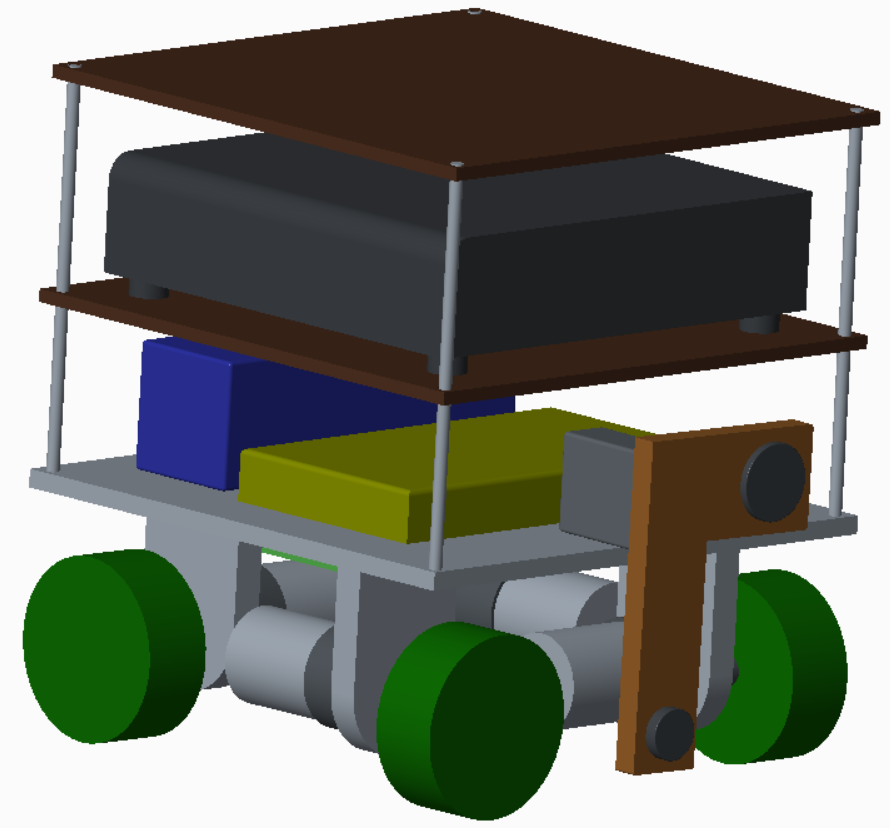
\includegraphics[width=0.95\textwidth]{fig/ROBOT.png}
   \caption{Repr�sentation 3D du robot}
   \label{f:CAD}
\end{figure}